\documentclass{standalone}
\usepackage{tikz}
\usetikzlibrary{patterns, positioning}

\begin{document}
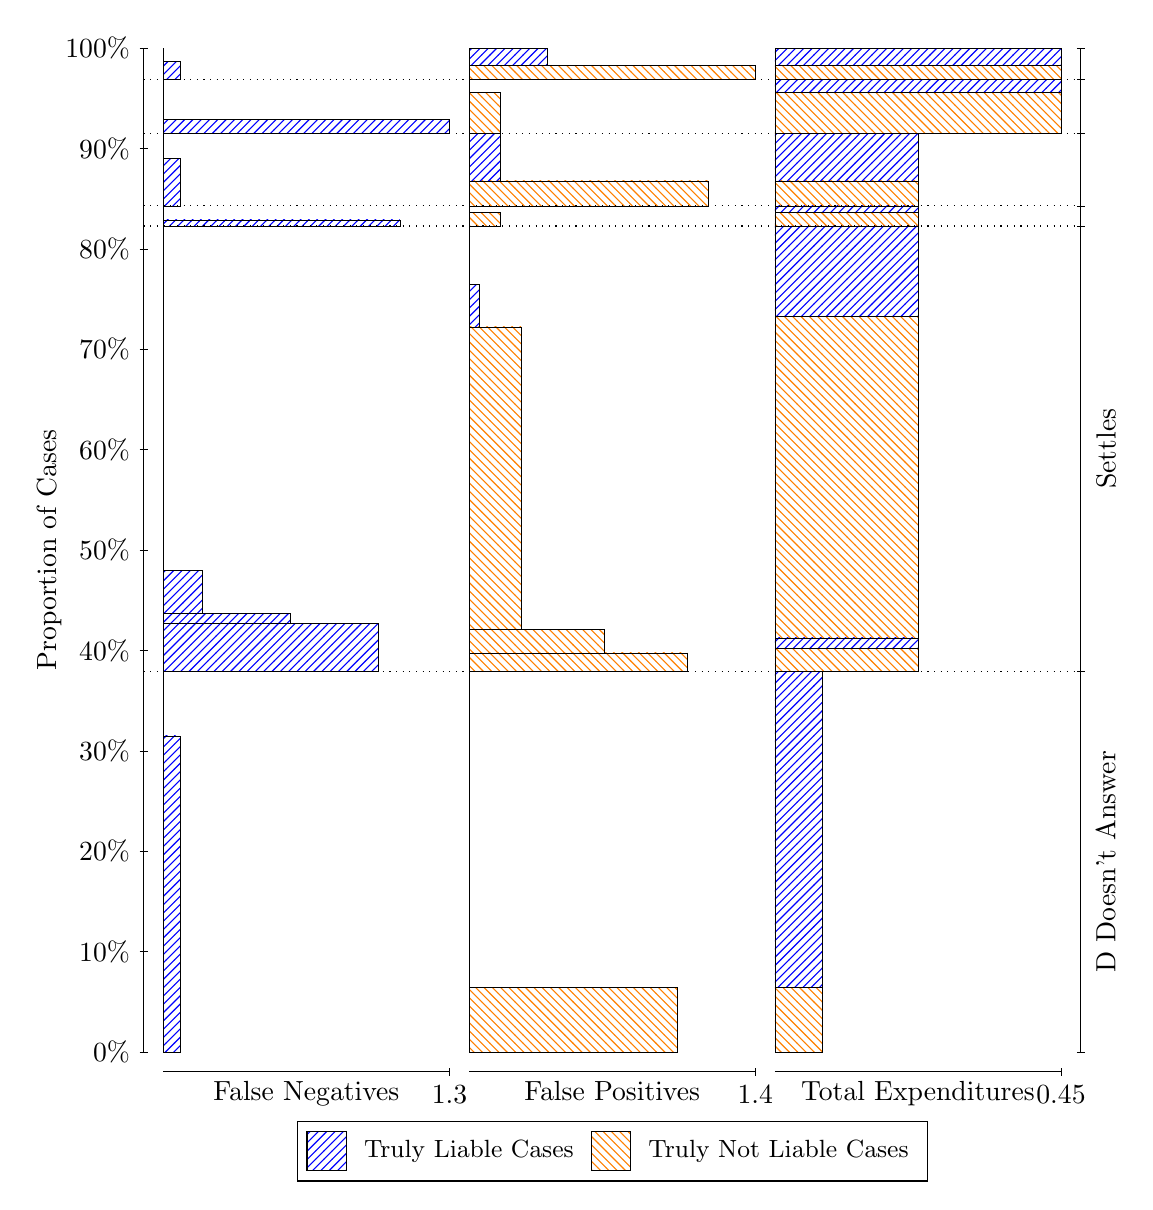
\begin{tikzpicture}
\draw[black, very thin] (1.5,1.75) -- (1.5,14.5);
\node[rotate=90, anchor=center] at (0.3, 8.125) {Proportion of Cases};
\draw[black, very thin] (1.45,1.75) -- (1.55,1.75);
\node[anchor=east] at (1.45, 1.75) {0\%};
\draw[black, very thin] (1.45,3.025) -- (1.55,3.025);
\node[anchor=east] at (1.45, 3.025) {10\%};
\draw[black, very thin] (1.45,4.3) -- (1.55,4.3);
\node[anchor=east] at (1.45, 4.3) {20\%};
\draw[black, very thin] (1.45,5.575) -- (1.55,5.575);
\node[anchor=east] at (1.45, 5.575) {30\%};
\draw[black, very thin] (1.45,6.85) -- (1.55,6.85);
\node[anchor=east] at (1.45, 6.85) {40\%};
\draw[black, very thin] (1.45,8.125) -- (1.55,8.125);
\node[anchor=east] at (1.45, 8.125) {50\%};
\draw[black, very thin] (1.45,9.4) -- (1.55,9.4);
\node[anchor=east] at (1.45, 9.4) {60\%};
\draw[black, very thin] (1.45,10.675) -- (1.55,10.675);
\node[anchor=east] at (1.45, 10.675) {70\%};
\draw[black, very thin] (1.45,11.95) -- (1.55,11.95);
\node[anchor=east] at (1.45, 11.95) {80\%};
\draw[black, very thin] (1.45,13.225) -- (1.55,13.225);
\node[anchor=east] at (1.45, 13.225) {90\%};
\draw[black, very thin] (1.45,14.5) -- (1.55,14.5);
\node[anchor=east] at (1.45, 14.5) {100\%};

\draw[black, very thin] (13.4,1.75) -- (13.4,14.5);
\draw[black, very thin] (13.35,1.75) -- (13.45,1.75);
\node[anchor=west] at (13.35, 1.75) {};
\draw[black, very thin] (13.35,6.5808) -- (13.45,6.5808);
\node[anchor=west] at (13.35, 6.5808) {};
\draw[black, very thin] (13.35,12.24) -- (13.45,12.24);
\node[anchor=west] at (13.35, 12.24) {};
\draw[black, very thin] (13.35,12.495) -- (13.45,12.495);
\node[anchor=west] at (13.35, 12.495) {};
\draw[black, very thin] (13.35,13.419) -- (13.45,13.419);
\node[anchor=west] at (13.35, 13.419) {};
\draw[black, very thin] (13.35,14.105) -- (13.45,14.105);
\node[anchor=west] at (13.35, 14.105) {};
\draw[black, very thin] (13.35,14.5) -- (13.45,14.5);
\node[anchor=west] at (13.35, 14.5) {};

\draw[black, very thin, pattern color=blue, pattern=north east lines] (1.75,1.75) rectangle (1.9596,5.7639);
\draw[black, very thin, pattern color=orange, pattern=north west lines] (1.75,5.7639) rectangle (1.75,6.5808);
\draw[black, very thin, pattern color=blue, pattern=north east lines] (1.75,6.5808) rectangle (4.475,7.193);
\draw[black, very thin, pattern color=blue, pattern=north east lines] (1.75,7.193) rectangle (3.3571,7.3233);
\draw[black, very thin, pattern color=blue, pattern=north east lines] (1.75,7.3233) rectangle (2.2391,7.8624);
\draw[black, very thin, pattern color=orange, pattern=north west lines] (1.75,7.8624) rectangle (1.75,12.24);
\draw[black, very thin, pattern color=blue, pattern=north east lines] (1.75,12.24) rectangle (4.7545,12.317);
\draw[black, very thin, pattern color=orange, pattern=north west lines] (1.75,12.317) rectangle (1.75,12.495);
\draw[black, very thin, pattern color=blue, pattern=north east lines] (1.75,12.495) rectangle (1.9596,13.101);
\draw[black, very thin, pattern color=orange, pattern=north west lines] (1.75,13.101) rectangle (1.75,13.419);
\draw[black, very thin, pattern color=blue, pattern=north east lines] (1.75,13.419) rectangle (5.3833,13.59);
\draw[black, very thin, pattern color=orange, pattern=north west lines] (1.75,13.59) rectangle (1.75,14.105);
\draw[black, very thin, pattern color=blue, pattern=north east lines] (1.75,14.105) rectangle (1.9596,14.329);
\draw[black, very thin, pattern color=orange, pattern=north west lines] (1.75,14.329) rectangle (1.75,14.5);
\draw[black, very thin, pattern color=orange, pattern=north west lines] (5.6333,1.75) rectangle (8.2758,2.5669);
\draw[black, very thin, pattern color=blue, pattern=north east lines] (5.6333,2.5669) rectangle (5.6333,6.5808);
\draw[black, very thin, pattern color=orange, pattern=north west lines] (5.6333,6.5808) rectangle (8.4079,6.817);
\draw[black, very thin, pattern color=orange, pattern=north west lines] (5.6333,6.817) rectangle (7.3509,7.1159);
\draw[black, very thin, pattern color=orange, pattern=north west lines] (5.6333,7.1159) rectangle (6.2939,10.958);
\draw[black, very thin, pattern color=blue, pattern=north east lines] (5.6333,10.958) rectangle (5.7655,11.497);
\draw[black, very thin, pattern color=blue, pattern=north east lines] (5.6333,11.497) rectangle (5.6333,12.24);
\draw[black, very thin, pattern color=orange, pattern=north west lines] (5.6333,12.24) rectangle (6.0297,12.417);
\draw[black, very thin, pattern color=blue, pattern=north east lines] (5.6333,12.417) rectangle (5.6333,12.495);
\draw[black, very thin, pattern color=orange, pattern=north west lines] (5.6333,12.495) rectangle (8.6721,12.813);
\draw[black, very thin, pattern color=blue, pattern=north east lines] (5.6333,12.813) rectangle (6.0297,13.419);
\draw[black, very thin, pattern color=orange, pattern=north west lines] (5.6333,13.419) rectangle (6.0297,13.933);
\draw[black, very thin, pattern color=blue, pattern=north east lines] (5.6333,13.933) rectangle (5.6333,14.105);
\draw[black, very thin, pattern color=orange, pattern=north west lines] (5.6333,14.105) rectangle (9.2667,14.276);
\draw[black, very thin, pattern color=blue, pattern=north east lines] (5.6333,14.276) rectangle (6.6242,14.5);
\draw[black, very thin, pattern color=orange, pattern=north west lines] (9.5167,1.75) rectangle (10.122,2.5669);
\draw[black, very thin, pattern color=blue, pattern=north east lines] (9.5167,2.5669) rectangle (10.122,6.5808);
\draw[black, very thin, pattern color=orange, pattern=north west lines] (9.5167,6.5808) rectangle (11.333,6.8797);
\draw[black, very thin, pattern color=blue, pattern=north east lines] (9.5167,6.8797) rectangle (11.333,7.0101);
\draw[black, very thin, pattern color=orange, pattern=north west lines] (9.5167,7.0101) rectangle (11.333,11.088);
\draw[black, very thin, pattern color=blue, pattern=north east lines] (9.5167,11.088) rectangle (11.333,12.24);
\draw[black, very thin, pattern color=orange, pattern=north west lines] (9.5167,12.24) rectangle (11.333,12.417);
\draw[black, very thin, pattern color=blue, pattern=north east lines] (9.5167,12.417) rectangle (11.333,12.495);
\draw[black, very thin, pattern color=orange, pattern=north west lines] (9.5167,12.495) rectangle (11.333,12.813);
\draw[black, very thin, pattern color=blue, pattern=north east lines] (9.5167,12.813) rectangle (11.333,13.419);
\draw[black, very thin, pattern color=orange, pattern=north west lines] (9.5167,13.419) rectangle (13.15,13.933);
\draw[black, very thin, pattern color=blue, pattern=north east lines] (9.5167,13.933) rectangle (13.15,14.105);
\draw[black, very thin, pattern color=orange, pattern=north west lines] (9.5167,14.105) rectangle (13.15,14.276);
\draw[black, very thin, pattern color=blue, pattern=north east lines] (9.5167,14.276) rectangle (13.15,14.5);
\draw[black, dotted] (1.5,6.5808) -- (13.4,6.5808);
\draw[black, dotted] (1.5,12.24) -- (13.4,12.24);
\draw[black, dotted] (1.5,12.495) -- (13.4,12.495);
\draw[black, dotted] (1.5,13.419) -- (13.4,13.419);
\draw[black, dotted] (1.5,14.105) -- (13.4,14.105);
\draw[black, very thin] (1.75,1.5) -- (5.3833,1.5);
\node[anchor=north] at (3.5667, 1.5) {False Negatives};
\draw[black, very thin] (5.3833,1.45) -- (5.3833,1.55);
\node[anchor=north] at (5.3833, 1.45) {1.3};

\draw[black, very thin] (5.6333,1.5) -- (9.2667,1.5);
\node[anchor=north] at (7.45, 1.5) {False Positives};
\draw[black, very thin] (9.2667,1.45) -- (9.2667,1.55);
\node[anchor=north] at (9.2667, 1.45) {1.4};

\draw[black, very thin] (9.5167,1.5) -- (13.15,1.5);
\node[anchor=north] at (11.333, 1.5) {Total Expenditures};
\draw[black, very thin] (13.15,1.45) -- (13.15,1.55);
\node[anchor=north] at (13.15, 1.45) {0.45};

\node[black, centered, rotate=90] at (13.72, 4.1654) {D Doesn't Answer};
\node[black, centered, rotate=90] at (13.72, 9.4101) {Settles};





\draw (7.449999999999999,1.5) node[draw=none] (baseCoordinate) {};
\begin{scope}[align=center]
        \matrix[scale=0.5, draw=black, below=0.5cm of baseCoordinate, nodes={draw}, column sep=0.1cm]{
            \node[rectangle, draw, minimum width=0.5cm, minimum height=0.5cm, pattern=north east lines, pattern color=blue] {}; &
            \node[draw=none, font=\small] (B) {Truly Liable Cases}; &
            \node[rectangle, draw, minimum width=0.5cm, minimum height=0.5cm, pattern=north west lines, pattern color=orange] {}; &
            \node[draw=none, font=\small] (B) {Truly Not Liable Cases}; \\
            };
\end{scope}

\end{tikzpicture}
\end{document}